\section{Data Overview}
\subsection{Dataset Description}
The Telco Customer Churn dataset contains information about telecommunications customers, with the primary objective of predicting customer churn. Churn refers to customers discontinuing their service with the company. By analyzing customer attributes, including demographics, service subscriptions, and billing details, businesses can identify patterns that may indicate a higher likelihood of churn.\\

This dataset is widely used for customer retention analysis, offering valuable insights into customer behavior and helping organizations develop data-driven strategies to improve customer loyalty. The dataset was originally provided by IBM and serves as a benchmark dataset for churn prediction in the telecom industry.

\subsection{Features}
The dataset consists of 7,043 records, each representing a unique customer, and includes 21 attributes that capture various aspects of a customer’s profile and service history. These attributes can be categorized into different groups:
\begin{itemize}
    \item \textbf{Customer Information:} These attributes provide demographic details about the customer, such as:
    \begin{itemize}
        \item customerID: A unique identifier assigned to each customer.
        \item gender: The gender of the customer.
        \item SeniorCitizen: A binary indicator (0 or 1) representing whether the customer is a senior citizen.
        \item Partner: Whether the customer has a partner.
        \item Dependents: Whether the customer has dependents.
    \end{itemize}
\end{itemize}
\begin{itemize}
    \item \textbf{Subscription Details:} These attributes describe the customer's subscription type and contract status:
    \begin{itemize}
        \item tenure: The number of months a customer has stayed with the company.
        \item Contract: The contract type (Month-to-month, One year, Two year).
        \item PaperlessBilling: Indicates whether the customer uses paperless billing.
        \item PaymentMethod: The customer's preferred payment method (Electronic check, Mailed check, Bank transfer, Credit card).
    \end{itemize}
    \item \textbf{Service Usage:} These attributes indicate the services subscribed to by the customer:
    \begin{itemize}
        \item PhoneService: Whether the customer has a phone service.
        \item MultipleLines: Whether the customer has multiple lines.
        \item InternetService: The type of internet service (DSL, Fiber optic, No service).
        \item OnlineSecurity: Whether the customer has online security services.
        \item OnlineBackup: Whether the customer has an online backup service.
        \item DeviceProtection: Whether the customer has device protection.
        \item TechSupport: Whether the customer has technical support.
        \item StreamingTV: Whether the customer has a streaming TV service.
        \item StreamingMovies: Whether the customer has a streaming movie service.
    \end{itemize}
    \item \textbf{Billing Information:} These attributes provide financial details of the customer's subscription:
    \begin{itemize}
        \item MonthlyCharges: The amount charged to the customer monthly.
        \item TotalCharges: The total amount charged to the customer over their tenure.
    \end{itemize}
    \item \textbf{Target Variable:}
    \begin{itemize}
        \item Churn: The dependent variable indicates whether the customer has churned (Yes/No).
    \end{itemize}
\end{itemize}
\subsection{Data Characteristics}

\begin{figure}[hbt!] 
    \centering
    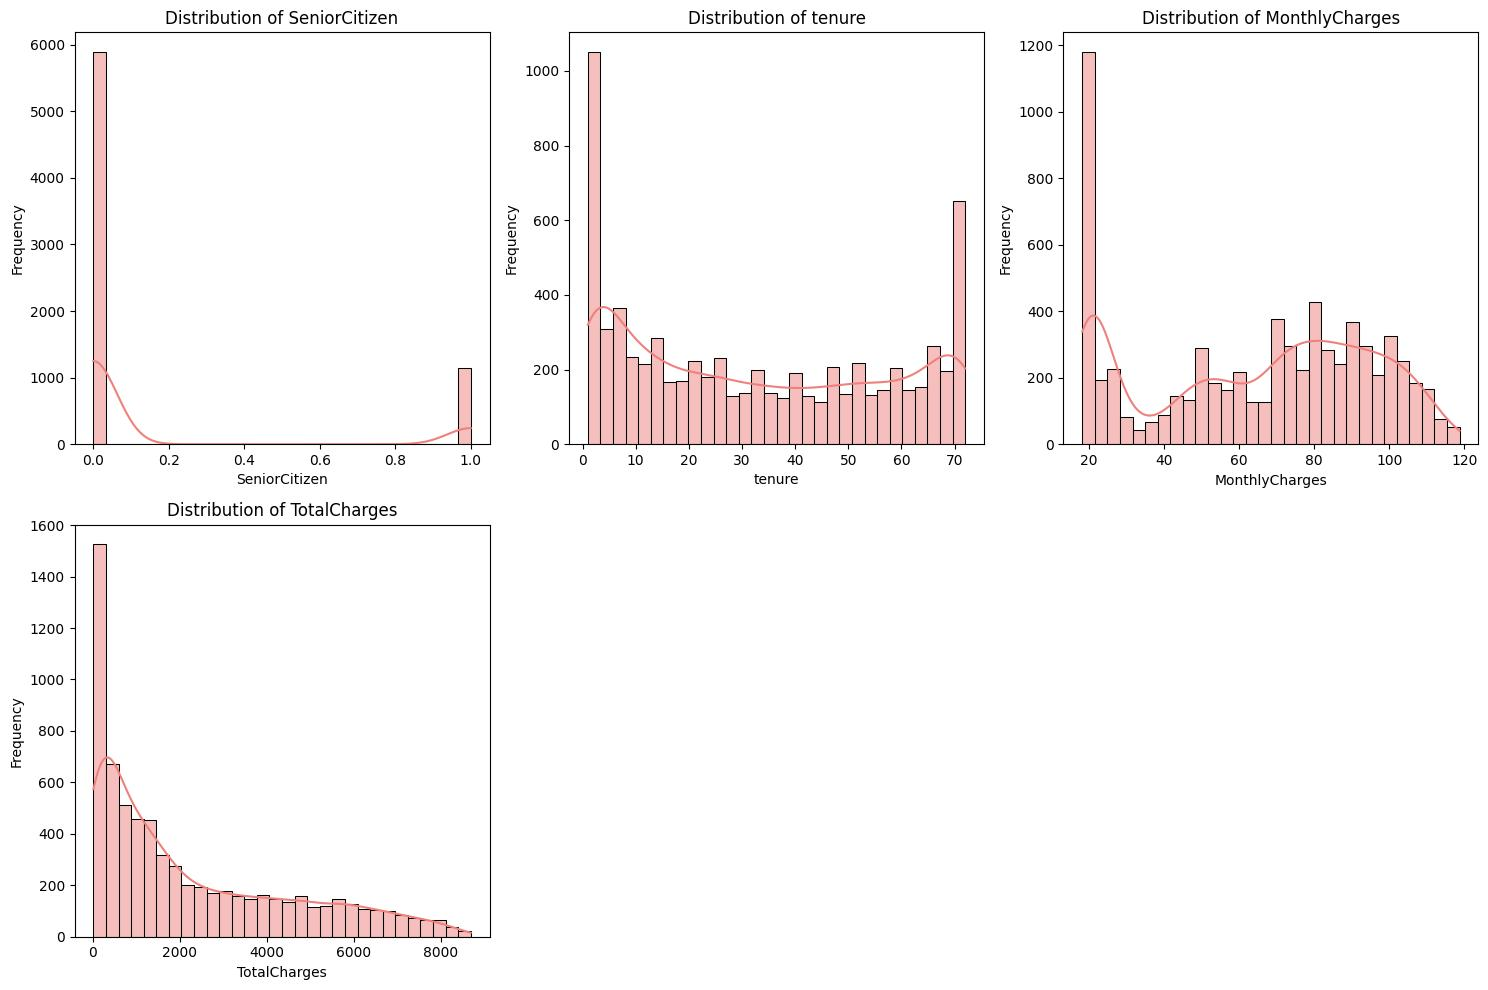
\includegraphics[width=1\linewidth]{Images/2.3.a.jpg}
    \caption{Distribution of Key Features in the Telco Customer Churn Dataset }
    \label{fig:enter-label}
\end{figure}

The histograms provide a comprehensive look at the distribution of key features in the Telco Customer Churn dataset. The SeniorCitizen variable is highly imbalanced, with most customers being non-senior citizens. This indicates that the dataset has a skewed demographic, with fewer senior customers. The tenure distribution shows a wide range of values, with notable peaks at specific points, suggesting that many customers have been with the company for just a few years. The MonthlyCharges distribution is bimodal, with peaks at around 20 and 80, likely reflecting two distinct customer groups: one with lower-cost subscriptions and another with higher-cost plans. Lastly, the TotalCharges distribution is right-skewed, with most customers having lower total charges, but a small group of long-term or high-value customers having significantly higher charges. These insights are valuable for preprocessing and feature engineering in predictive models for customer churn.\\

\begin{figure}[hbt!]
    \centering
    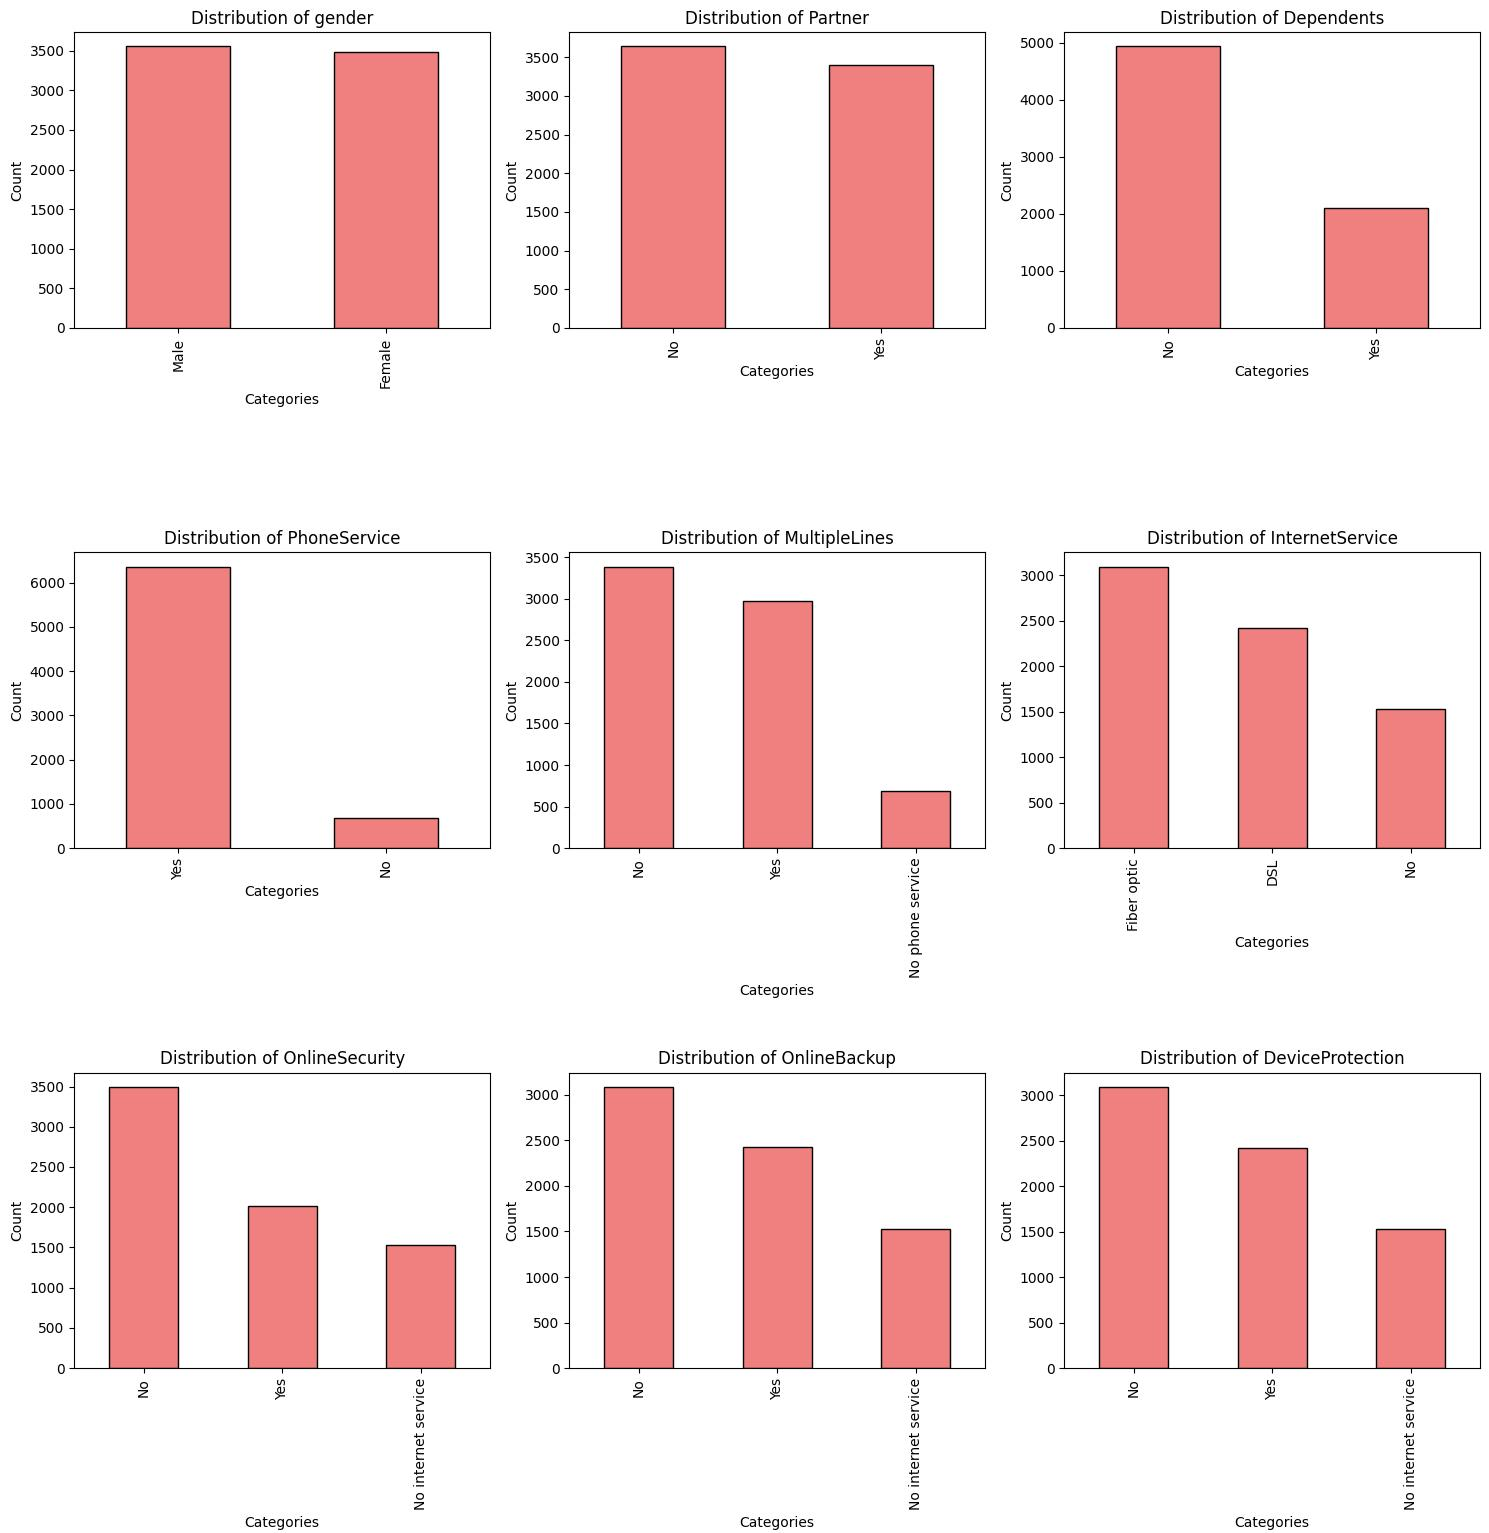
\includegraphics[width=1\linewidth]{Images/2.3.b.jpg}
    \caption{Distribution of Categorical Features in the Telco Customer Churn Dataset }
    \label{fig:enter-label}
\end{figure}

The bar charts give an overview of the categorical features in the dataset. The gender distribution is nearly balanced between male and female customers. However, a large proportion of customers do not have partners or dependents, as seen in the Partner and Dependents distributions. Regarding service features, most customers have PhoneService, but fewer have MultipleLines. The majority of customers use fiber optic or DSL for internet, while a smaller proportion do not have internet service at all. \\

\begin{figure}[hbt!]
    \centering
    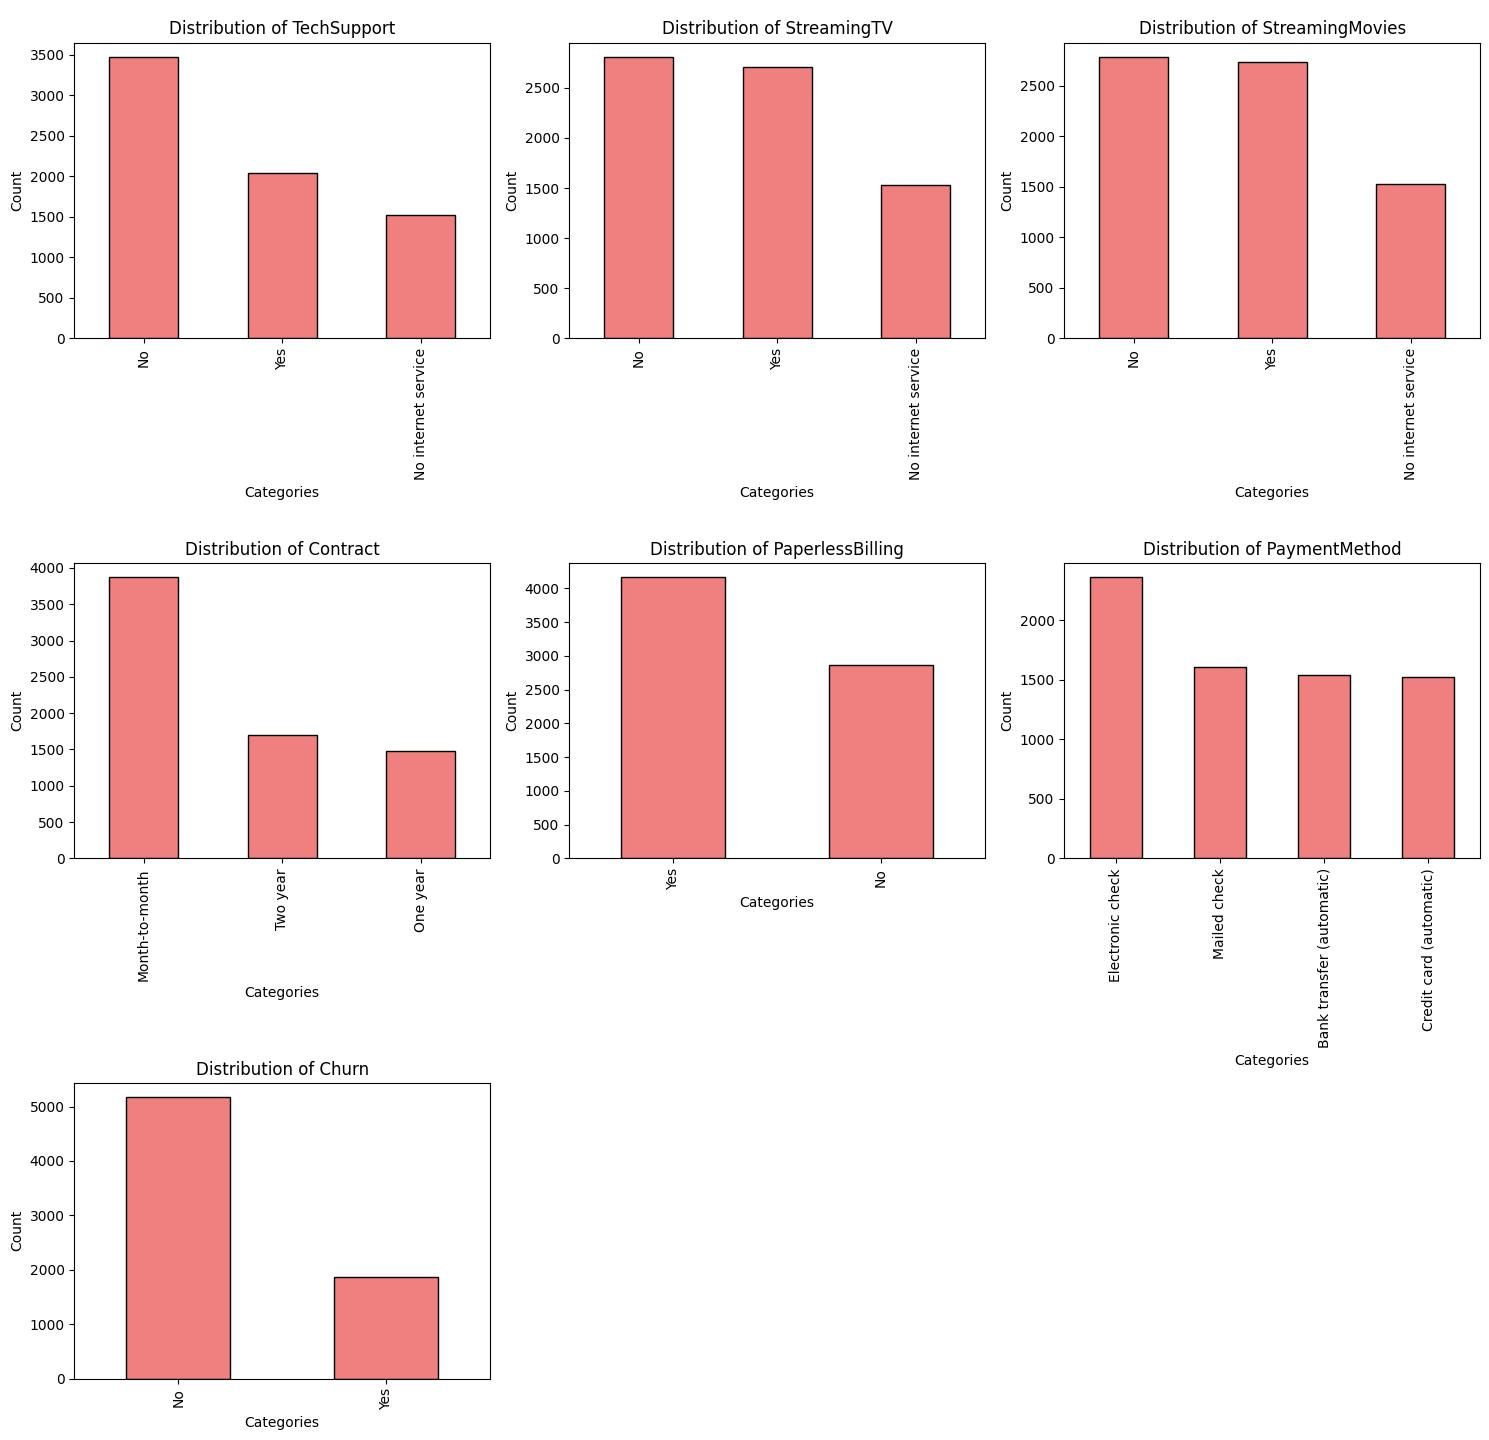
\includegraphics[width=1\linewidth]{Images/2.3.c.jpg}
    \caption{Distribution of Categorical Features in the Telco Customer Churn Dataset }
    \label{fig:enter-label}
\end{figure}

Additionally, many customers do not use add-on services like OnlineSecurity, OnlineBackup, DeviceProtection, or Streaming services, which may suggest limited engagement with premium features. Most customers are on month-to-month contracts, and a large proportion use paperless billing. As for payment methods, electronic checks are the most common, followed by mailed checks and bank transfers. Finally, the Churn distribution shows that most customers stay with the company, with a smaller number deciding to leave. These observations can help inform future analyses and model development aimed at predicting customer churn.\\

\begin{figure}[hbt!]
    \centering
    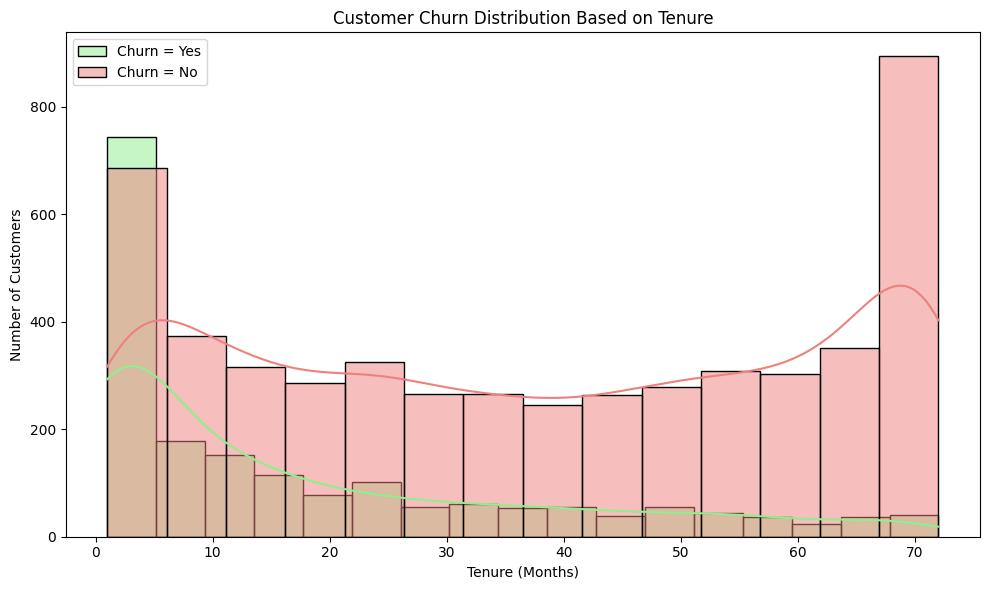
\includegraphics[width=1\linewidth]{Images/2.3.d.jpg}
    \caption{Customer Churn Distribution Based on Tenure}
    \label{fig:enter-label}
\end{figure}

The chart showing the relationship between churn and tenure reveals that churn is highest in the first few months of a customer’s subscription, with many customers leaving early. As the tenure increases, the number of churned customers drops significantly, indicating that long-term customers are far less likely to cancel their services. This suggests that the company has a higher retention rate among long-term customers, possibly due to factors like customer satisfaction or loyalty programs. The trend underscores the importance of focusing on customer retention in the early stages of subscription, as customers who stay longer are more likely to remain with the company.\\

\begin{figure}[hbt!]
    \centering
    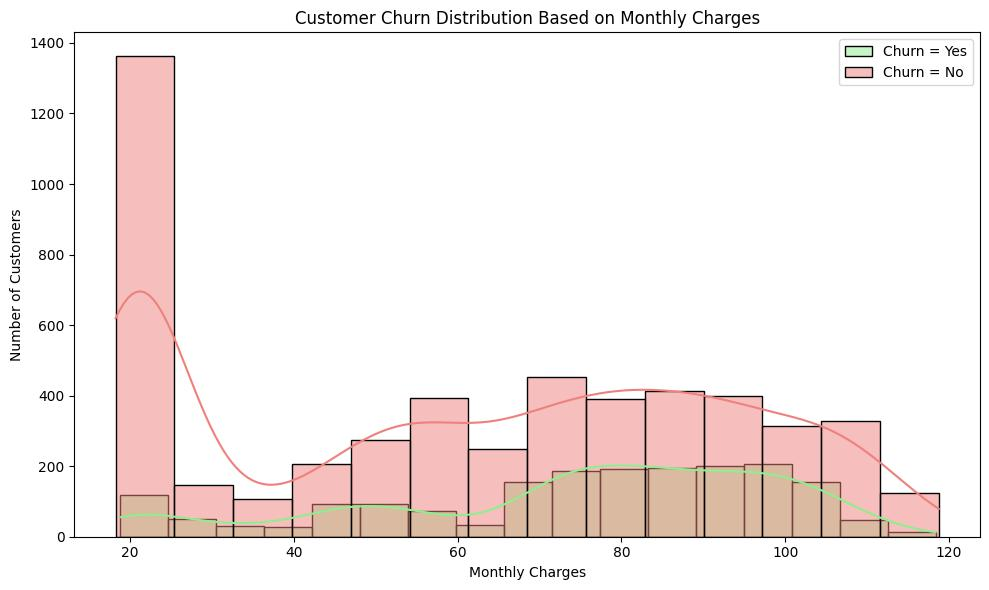
\includegraphics[width=1\linewidth]{Images/2.3.e.jpg}
    \caption{Customer Churn Distribution  Based on Monthly Charges}
    \label{fig:enter-label}
\end{figure}

In the chart illustrating the relationship between churn and monthly charges, we see that customers with lower monthly charges (around 20) tend to stay with the service, as indicated by the higher bar and lower churn rate in this range. Conversely, as monthly charges increase, the likelihood of churn also rises. This suggests that customers with higher monthly charges may be more sensitive to the perceived value of the service or may find better alternatives from competitors, leading to a higher churn rate among this group. The trend highlights the importance of carefully managing pricing plans, particularly for customers with higher charges, to reduce the risk of churn.

\subsection{Data Preprocessing}
Data preprocessing is a crucial step in preparing the dataset for machine learning models. It ensures that all features are formatted correctly, handles any missing values, and encodes categorical variables properly. The preprocessing steps performed in this study are described below.\\

We begin by storing the data in a pandas DataFrame, which allows for efficient manipulation and analysis. The dataset is loaded using the read\_csv function.

\subsubsection{Data Cleaning}
The first step in cleaning the data is to remove the customerID column. This column only serves as an identifier and does not contribute to the predictive analysis, so removing it helps simplify the dataset and ensures that irrelevant information doesn't negatively impact the model's performance.\\

Next, we address an issue with the TotalCharges column. While this column should be numerical, it is stored as an object (string). Upon inspection, we found that some values in this column were blank spaces instead of numerical data. Since there were only 11 missing values out of 7,043 records, we decided to remove these rows rather than attempt to impute the missing values, which helps maintain the integrity of the data.

\subsubsection{Handling Missing Values}
The dataset was checked for missing values using the df.isnull().sum() method, and the results confirmed that all columns have zero missing values. This means the dataset is complete and free of missing data, which is essential for building accurate and reliable machine learning models.

\subsubsection{Feature Engineering}
Feature engineering is done to enhance the predictive power of the models. We begin by creating a new feature, tenure group, which categorizes customers based on their tenure duration, helping the model understand different customer segments.\\

We also examine categorical columns and their unique values. Many columns, such as Partner and Dependents, contain binary values like Yes and No, so we convert these into numerical representations (1 for Yes and 0 for No) to make them compatible with machine learning models. Additionally, some variables contain values like "No internet service" or "No phone service," which we standardize to just "No" for consistency across these columns.\\

For the gender variable, we map "Female" to 1 and "Male" to 0. Boolean columns are also converted into integers, where True becomes 1 and False becomes 0. We apply this transformation to all boolean columns in the dataset to simplify processing while preserving interpretability.\\

For categorical variables with more than two unique values (e.g., InternetService, Contract, and PaymentMethod), we use One-Hot Encoding. This technique converts each categorical feature into multiple binary columns, ensuring that no unintended ordinal relationships are introduced, which makes the data ready for machine learning models.

\subsubsection{Feature Scaling}
Since machine learning models can be sensitive to features with different scales, we apply Min-Max Scaling to normalize the numerical features. Columns such as tenure, MonthlyCharges, and TotalCharges have values that span a wide range, so scaling these features ensures they all contribute proportionally to the model’s learning process. Min-Max Scaling transforms these values to a range between 0 and 1.\\

\begin{figure}[hbt!]
    \centering
    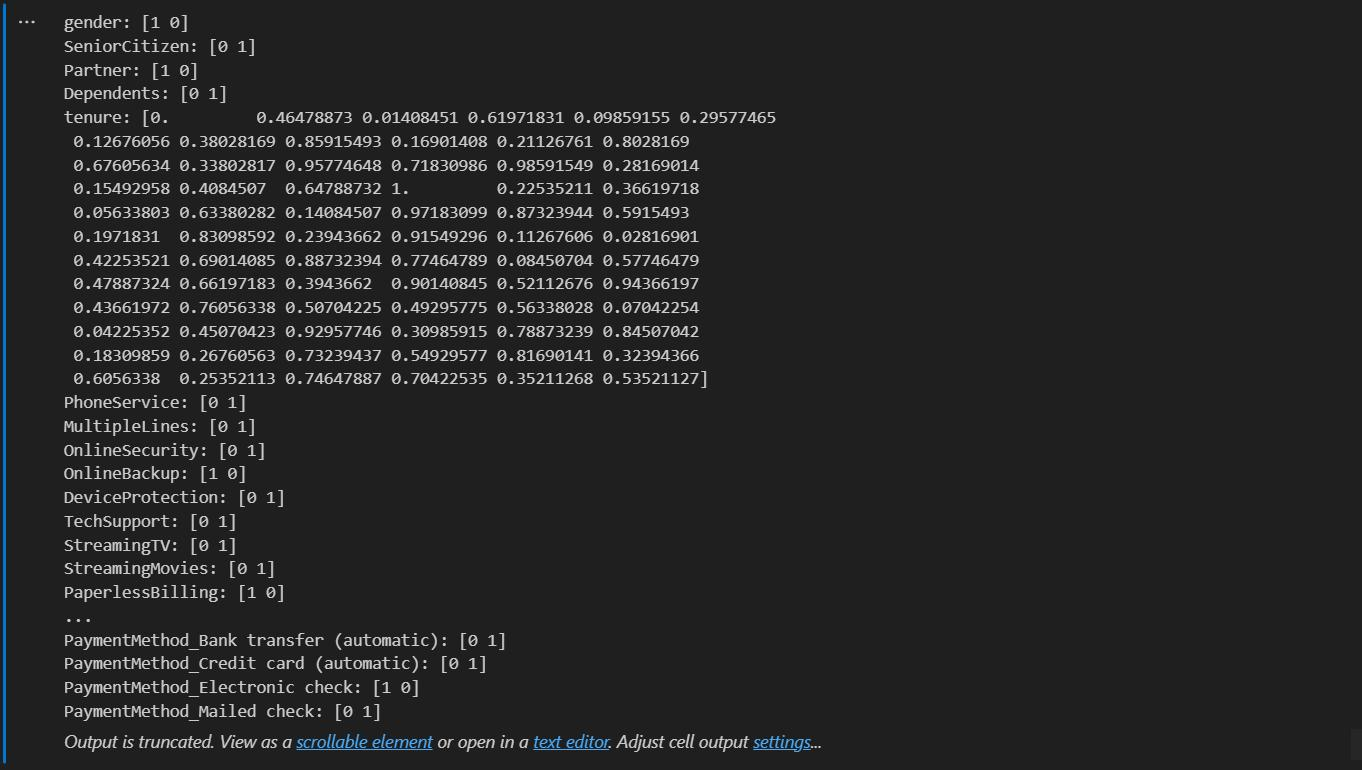
\includegraphics[width=1\linewidth]{Images/2.4.4.a.jpg}
    \caption{Feature Scaling Applied to the Dataset }
    \label{fig:enter-label}
\end{figure}

Finally, after completing the preprocessing steps, we validate the transformed dataset by checking the unique values in the categorical columns. This final check ensures that all transformations have been applied correctly and that the dataset is ready for training without any inconsistencies.

